\documentclass[a4paper,12pt]{article}
\usepackage[super,square]{natbib}
\usepackage{anysize}
\usepackage{amsmath}
\usepackage{amssymb}
\marginsize{2cm}{2cm}{1cm}{2cm}
\usepackage{fancyhdr}
\renewcommand{\headrulewidth}{0pt}
\usepackage{soul}
\usepackage[dvipsnames]{xcolor}
\usepackage{hyperref}
\usepackage{graphicx}
\usepackage{float}
\hypersetup{
    colorlinks=true,
    linkcolor=black,
    citecolor=CadetBlue,
    filecolor=CadetBlue,      
    urlcolor=CadetBlue,
}
\usepackage{lipsum}
\usepackage{multicol}
\usepackage{parskip}
\usepackage{listings}
\usepackage{xcolor}
\lstset{
  language=Python,
  basicstyle=\ttfamily\footnotesize,
  numbers=left,
  numberstyle=\tiny\color{gray},
  frame=single,
  breaklines=true,
  breakatwhitespace=false,
  tabsize=4,
  showspaces=false,
  showstringspaces=false,
  showtabs=false,
  captionpos=b,
  backgroundcolor=\color{lightgray!10},
  commentstyle=\color{green!60!black}\textit,
  keywordstyle=\color{blue},
  stringstyle=\color{red}
}
\setlength\columnsep{18pt}
\renewenvironment{abstract}
 {\par\noindent\textbf{\abstractname}\ \ignorespaces \\}
 {\par\noindent\medskip}
\renewcommand{\abstractname}{Question}
 
\begin{document}
\pagestyle{fancy}
\thispagestyle{empty}
\fancyhead[R]{\textit{EE1060 - Quiz 03}}
\fancyhead[L]{}
\renewcommand*{\thefootnote}{\fnsymbol{footnote}}
\begin{center}
\Large{\textbf{EE1060 \\ Differential Equations And Transform Techniques \\ Quiz 03}}
\vspace{0.4cm}
\normalsize
\\ Submission by Team 08 \\
\vspace{0.1cm}
\textit{IIT Hyderabad}
\medskip
\normalsize
\end{center}
{\color{gray}\hrule}
\vspace{0.4cm}
\begin{abstract}
Compute the response of a series $RL$ circuit to a square wave input as shown in Fig.~\ref{input_wave}, both numerically and analytically. For the numerical approach, use appropriate numerical techniques to solve the differential equation governing the $RL$ circuit's behaviour. For the analytical approach, utilise Fourier Series to derive the response of the circuit. The square wave is characterised by a duty ratio, denoted by the factor $\alpha$. You are free to choose the values of resistance $R$ and inductance $L$ for your analysis.

\begin{figure}[H]
  \centering
  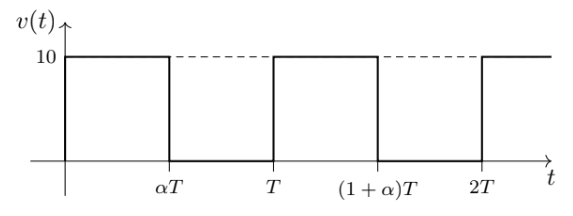
\includegraphics[width=0.5\textwidth]{input_wave.png}
  \caption{Square wave with a duty ratio $\alpha$}
  \label{input_wave}
\end{figure}

Analyse the circuit's behaviour obtained from both numerical and analytical methods. In your analysis, apply the relevant concepts from the course related to circuits and differential equations to explore the response and draw comparisons between the two approaches.

\end{abstract}
{\color{gray}\hrule}
\medskip
\newpage
\begin{multicols}{2}
\tableofcontents
\end{multicols}
\newpage

{\color{gray}\hrule}
\begin{center}
\section{Decomposing the Input Wave Into Fourier Series}
\bigskip
\end{center}
{\color{gray}\hrule}
\begin{multicols}{2}

To analyse the circuit response, we express the input signal using Fourier Series. This can be done in two ways.

\subsection{Complex Exponential Form}
The Fourier series of a periodic function \( f(x) \) with period \( T \) can be expressed as:
\begin{align}
f(x) = \sum_{n=-\infty}^{\infty} c_n e^{j \frac{2\pi n}{T} x}  
\end{align}
where the Fourier coefficients \( c_n \) are given by:
\begin{align}
c_n = \frac{1}{T} \int_{0}^{T} f(x) e^{-j \frac{2\pi n}{T} x} \, dx \label{1}
\end{align}

\subsection{Trigonometric Form}
The Fourier series can also be written (for real signals) in terms of sinusoidal terms as:
\begin{equation}
\begin{split}
f(x) &= a_0 + \sum_{n=1}^{\infty} \left[ a_n \cos\left(\frac{2\pi n}{T} x \right) \right. \\
&+ \sum_{n=1}^{\infty} \left[ b_n \sin\left(\frac{2\pi n}{T} x \right) \right]
\end{split}
\end{equation}
where the coefficients are given by:
\begin{align}
a_0 = \frac{1}{T} \int_{0}^{T} f(x) \, dx \label{2}
\end{align}
\begin{align}
a_n =c_n+c_{-n} = \frac{2}{T} \int_{0}^{T} f(x) \cos\left(\frac{2\pi n}{T} x \right) \, dx \label{3}
\end{align}
\begin{align}
b_n = j(c_n-c_{-n}) =\frac{2}{T} \int_{0}^{T} f(x) \sin\left(\frac{2\pi n}{T} x \right) \, dx \label{4}
\end{align}
We will use the notation $\omega_0$ to represent $\frac{2\pi}{T}$ going forward.

\subsection{Orthogonality Property of Terms}
Considering the complex form of Fourier series, the complex coefficients can be computed as:
\begin{align}
c_n = \frac{1}{T} \int_{0}^{T} f(x) e^{-j \frac{2\pi n}{T} x} \, dx 
\end{align}
In the complex Fourier series, the set of exponential functions:
\[
e^{j \frac{2\pi n}{T} x}, \quad n \in \mathbb{Z}
\]
forms an orthogonal set over the interval \( [0, T] \) with respect to the inner product:
\[
\langle f, g \rangle = \int_{0}^{T} f(x) \overline{g(x)} \, dx.
\]
For any integers \( m \) and \( n \), the orthogonality property is given by:
\[
\int_{0}^{T} e^{j \frac{2\pi m}{T} x} \cdot e^{-j \frac{2\pi n}{T} x} \, dx
= \int_{0}^{T} e^{j \frac{2\pi (m-n)}{T} x} \, dx
\]
which evaluates to:
\[
\begin{cases}
T, & \text{if } m = n \\
0, & \text{if } m \neq n
\end{cases}
\]
Thus, the complex exponentials \( e^{j \frac{2\pi n}{T} x} \) form an \textbf{orthonormal basis} in the space of periodic functions.

\subsection{Fourier Series Representation of the Given Square Input Wave}
Substituting the value of $f(x)$ in (\ref{1}) and computing $C_k$, we get:
\begin{align}
C_k &= \frac{1}{T} \int_{0}^{T} f(t) e^{-j k \omega_0 t} dt\\
&= \frac{1}{T} \left( \int_{0}^{\alpha T} 10 \cdot e^{-j k \omega_0 t} dt+ 0\right)\\
&= \frac{10}{T} \left( \frac{e^{-j k \omega_0 \alpha T} - 1}{-j k \omega_0} \right)\\
C_k &= \frac{10 j}{2 \pi k} [\cos 2 \pi k \alpha - j \sin 2 \pi k \alpha - 1]\\ 
&= \frac{5  \sin (2 \pi k \alpha)}{ \pi k} + j \left[ \frac{5}{ \pi k} (\cos 2 \pi k \alpha -1) \right]
\end{align}
From (\ref{2}), (\ref{3}) and (\ref{4}), we can compute the trigonometric coefficients of the Fourier Series.
\begin{align}
a_k &= C_k + C_{-k} \\
&= \frac{10 \sin( 2 \pi k \alpha)}{\pi k} \\
b_k &= j \{ C_k - C_{-k} \} \\
&= j \left( 2 j \right) \frac{5}{ \pi k} [\cos 2 \pi k \alpha - 1]\\
&=\left( \frac{10}{ \pi k} \right) \{1 - \cos 2 \pi k \alpha\}\\
a_0 = C_0 &= \frac{1}{T} \int_{0}^{T} f(t) dt \\
&= \frac{1}{T} \int_{0}^{\alpha T} 10 dt \\
&= \frac{10\alpha T}{T} = 10\alpha
\end{align}
Therefore, the Fourier Series representation of the given input wave is given by: 
\begin{equation}
\begin{split}
f(x) &= 10\alpha + \sum_{n=1}^{\infty} \Bigg[ \frac{10 \sin (2 \pi n \alpha)}{\pi n} \cos\left(\frac{2\pi n}{T} x \right) \\
&+ \frac{10}{\pi n} (1 - \cos (2 \pi n \alpha)) \sin\left(\frac{2\pi n}{T} x \right) \Bigg]
\end{split}
\end{equation}

\subsection{Verification}
To verify that the square wave was decomposed correctly into its Fourier Series, we will write a Python program to plot the calculated expression using the first 10000 terms. \\
\begin{figure}[H]
  \centering
  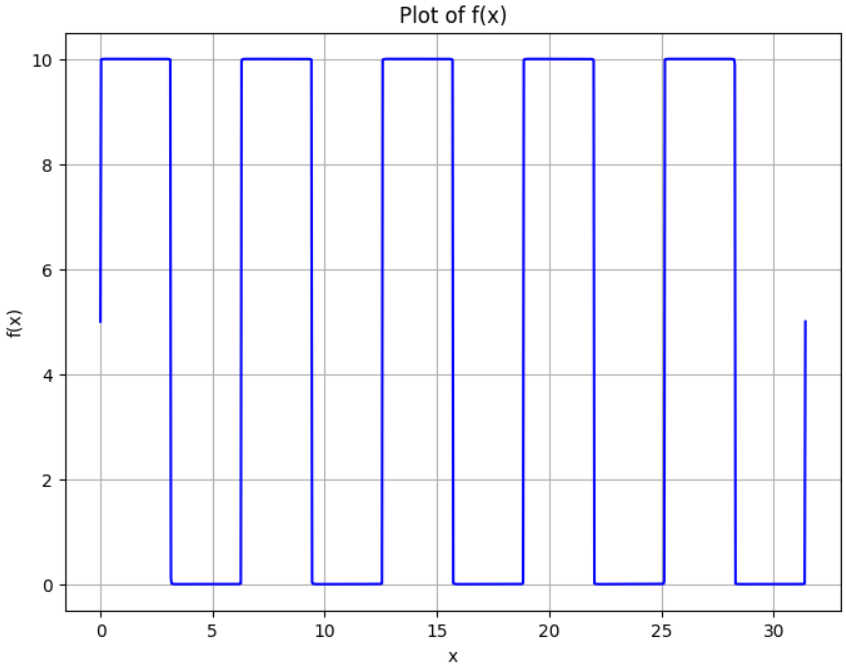
\includegraphics[width=\columnwidth]{sections/1_plot.png}
  \caption{Plot Generated Using Calculated Fourier Series Expression}
\end{figure}

\subsection{Magnitude Spectrum of $C_k$}
The magnitude spectrum is obtained by computing $|C_k|$ for different values of $k$. It provides insight into how much of each frequency component is present in the signal:
\begin{equation}
    |C_k| = \sqrt{\operatorname{Re}(C_k)^2 + \operatorname{Im}(C_k)^2}.\\
\end{equation}
The magnitude spectrum plots $|C_k|$ against $k$.

for the given input wave, $|C_k|$ is 
\begin{equation}
    |C_k| =\frac{5}{\pi k}\left(\sqrt{2(1-cos(2\pi k\alpha)} \right)
\end{equation}

\begin{figure}[H]
  \centering
  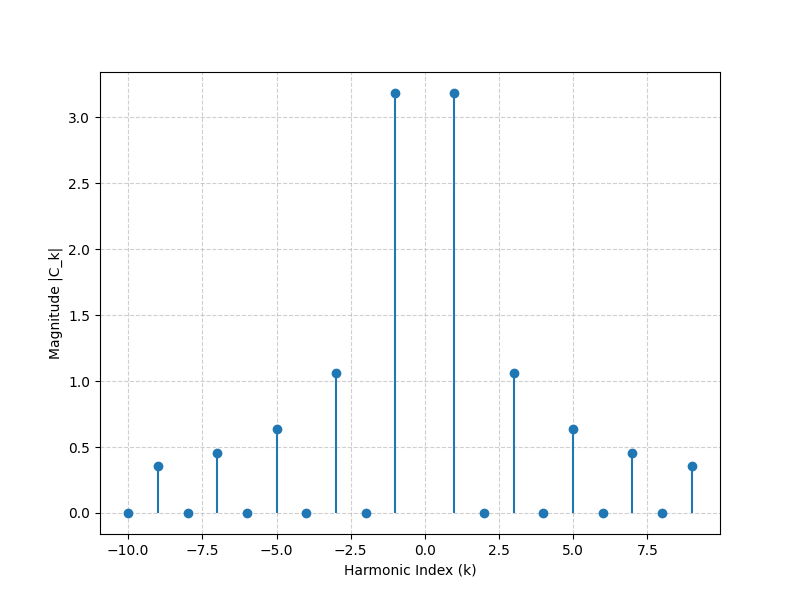
\includegraphics[width=\columnwidth]{sections/1_spectrum.png}
  \caption{For alpha=0.5}
\end{figure}
\begin{figure}[H]
  \centering
  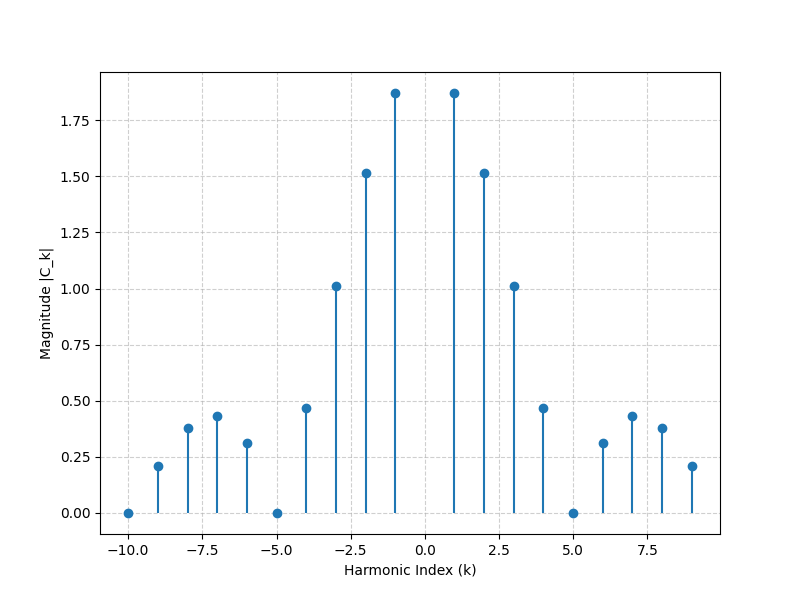
\includegraphics[width=\columnwidth]{sections/1_spectrum2.png}
  \caption{For alpha=0.2}
\end{figure}
\begin{figure}[H]
  \centering
  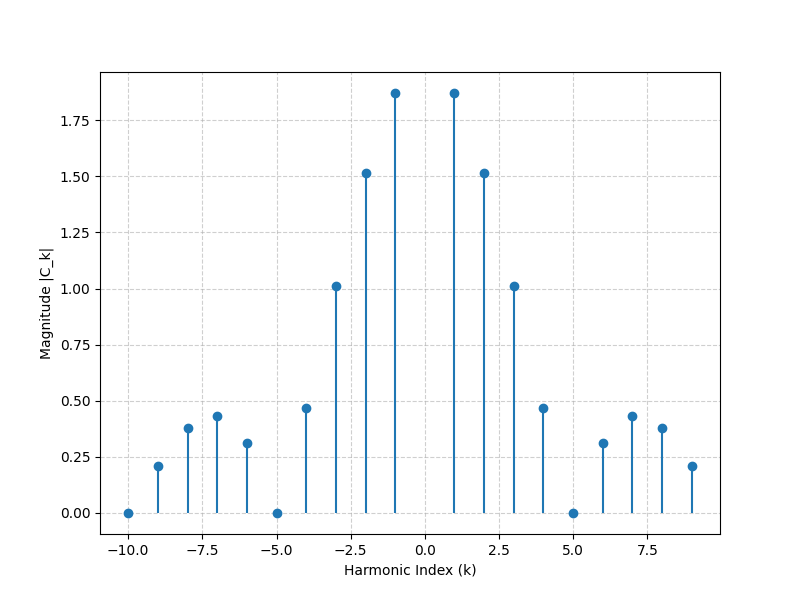
\includegraphics[width=\columnwidth]{sections/1_spectrum3.png}
  \caption{For alpha=0.8}
\end{figure}

\end{multicols}

\newpage
{\color{gray}\hrule}
\begin{center}
\section{Deducing the Differential Equation}
\bigskip
\end{center}
{\color{gray}\hrule}
\begin{multicols}{2}

\subsection{Defining the Square Wave}
The square wave \(v(t)\) alternates between two values, \(V_0\) and 0, with a period \(T\). The duty ratio \(\alpha\) determines the fraction of the period during which the voltage is \(V_0\). Specifically:
\begin{itemize}
    \item For \(0 \leq t < \alpha T\), \(v(t) = V_0\).
    \item For \(\alpha T \leq t < T\), \(v(t) = 0\).
\end{itemize}

\subsection{The Differential Equation for a Series RL Circuit}
The voltage across a series RL circuit is given by Kirchhoff's Loop Law as:
\[
v(t) = L \frac{di(t)}{dt} + R i(t)
\]
where \(i(t)\) is the current through the circuit.

\subsection{Solving the Differential Equation}
We need to solve this equation for two intervals:
\begin{enumerate}
    \item When \(v(t) = V_0=10\) (for \(0 \leq t < \alpha T\)):
    \begin{align}
        V_0 = L \frac{di(t)}{dt} + R i(t)\\
        \implies\frac{di(t)}{dt}+\frac{R}{L}i(t) =\frac{10}{L}
    \end{align}
    Integrating Factor $= e^{\int \frac{R}{L}dt}\implies e^{\frac{Rt}{L}}$\\
    Multiply both sides by the integrating factor and integrate.\\
    \begin{align}
        \int d(e^{\frac{Rt}{L}}i(t))&=\int e^{\frac{Rt}{L}}\frac{10}{L}dt\\
        e^{\frac{Rt}{L}}i(t) &= \frac{10}{L}\frac{e^{\frac{Rt}{L}}}{\frac{R}{L}} + C
    \end{align}
    Divide both sides with $e^{\frac{Rt}{L}}$
    \begin{align}
        i(t)&=\frac{10}{R} +Ce^{-\frac{Rt}{L}} \label{eq5}
    \end{align}
    Apply initial condition  $i(0)$ at $t=0$\\
    \begin{align}
        i(0)&=\frac{10}{R} +C\\
        C&=i(0)-\frac{10}{R} \label{eq7}
    \end{align}
    equation (\ref{eq7}) in (\ref{eq5}),
    \begin{align}
       i(t) &= \frac{10}{R} \left(1 - e^{-\frac{R}{L}t}\right) + i(0) e^{-\frac{R}{L}t}\\
       \text{since $i(0)=0$}\\
       i(t) &= \frac{10}{R} \left(1 - e^{-\frac{R}{L}t}\right)
    \end{align}
    \item When \(v(t) = 0\) (for \(\alpha T \leq t < T\)):
    \begin{align}
        0 = L \frac{di(t)}{dt} + R i(t)
    \end{align}
    The solution to this DE is:
    \begin{align}
        i(t) = i(\alpha T) e^{-\frac{R}{L}(t - \alpha T)}
    \end{align}
    where \(i(\alpha T)\) is the current at \(t = \alpha T\).
\end{enumerate}

\end{multicols}

\newpage
{\color{gray}\hrule}
\begin{center}
\section{The Analytical Solution}
\bigskip
\end{center}
{\color{gray}\hrule}
\begin{multicols}{2}

As discussed in the previous section, the given voltage input can also be expressed as a linear combination of DC and AC voltage sources, with the help of Fourier Series.
Thus we can interpret the differential equations of the system as
%\begin{align*}
    $L\frac{di}{dt}+Ri=f(x)$
%\end{align*}
where
\begin{equation}
\begin{split}
f(x) &= 10\alpha + \sum_{n=1}^{\infty} \Bigg[ \frac{10 \sin (2 \pi n \alpha)}{\pi n} \cos\left(\frac{2\pi n}{T} x \right) \\
&+ \frac{10}{\pi n} (1 - \cos (2 \pi n \alpha)) \sin\left(\frac{2\pi n}{T} x \right) \Bigg]
\end{split}
\end{equation}

\subsection{Current Response of the Circuit for Individual Inputs}

\subsubsection{For DC Voltage Input}
Assume the current produced in the circuit by the DC source to be $i_0$
The differential equation for this system is:

\begin{align}
    \frac{di_0}{dt}+\frac{R}{L}i_0=\frac{a_0}{L}
\end{align}
Multiplying with Integrating Factor $e^{\int \frac{R}{L}dt}=e^{\frac{R}{L}t}$ and integrating on both sides with limits $t=0$ to $t=t$, and considering $i_0(0)=0$,

\begin{align}
    i_0(t)=\frac{a_0}{R} \left(1-e^{\frac{-R}{L}t} \right)
\end{align}
where $a_0=10\alpha$.

\subsubsection{For AC Voltage Input}
Assume the current produced in the circuit by the AC source  $a_ncos(n\omega_0t)+b_nsin(n\omega_0t)$ to be $i_n$.\\
The differential equation for this system is:
\begin{align}
    \frac{di_n}{dt}+\frac{R}{L}i_n=\frac{a_n}{L}cos(n\omega_0t)+\frac{b_n}{L}sin(n\omega_0t)
\end{align}
Multiplying with Integrating Factor $e^{\int \frac{R}{L}dt=e^\frac{R}{L}t}$ and integrating on both sides with limits $t=0$ to $t=t$, and considering $i_n(0)=0$,
\begin{align}
e^{\frac{R}{L}t}i_n(t) &= \int_{0}^{t} e^{\frac{R}{L}t} \left( \frac{a_n}{L}\cos(n\omega_0t) \right) dt \nonumber \\
&+ \int_{0}^{t} e^{\frac{R}{L}t} \left( \frac{b_n}{L}\sin(n\omega_0t) \right) dt \label{eq}
\end{align}
Rewriting $a_ncos(n\omega_0t)+b_nsin(n\omega_0t)$ on RHS as 
\begin{align*}
    &=a_ncos(n\omega_0t)+b_nsin(n\omega_0t)\\
    &= \sqrt{a_n^2+b_n^2} \Bigg( \frac{a_n}{\sqrt{a_n^2+b_n^2}} \cos(n\omega_0t) \\
    &+ \frac{b_n}{\sqrt{a_n^2+b_n^2}} \sin(n\omega_0t) \Bigg)\\
    &=\sqrt{a_n^2+b_n^2}\left(cos(n\omega_0t-\phi) \right)\\
    &=\sqrt{a_n^2+b_n^2}\left( \frac{e^{j(n\omega_0t-\phi)}+e^{j(\phi-n\omega_0t)}}{2}\right)
\end{align*}
where $\phi=tan^{-1}\left(\frac{b_n}{a_n} \right)$ and substituting it back in (\ref{eq}), on RHS side we get
\begin{align}
    &=\frac{\sqrt{a_n^2+b_n^2}}{2L}\int_{0}^{t}\left( e^{\frac{R}{L}t+j(n\omega_0t-\phi)} + e^{\frac{R}{L}t+j(\phi-n\omega_0t)} \right)
\end{align}
After integrating, we get
\begin{align}
e^{\frac{R}{L}t}i_n(t) &= \frac{\sqrt{a_n^2+b_n^2}}{2L} \Bigg( \frac{e^{-j\phi}\left(e^{(\frac{R}{L}+jn\omega_0)t}-1 \right)}{\frac{R}{L}+jn\omega_0} \\
&+ \frac{e^{j\phi}\left(e^{(\frac{R}{L}-jn\omega_0)t}-1\right)}{\frac{R}{L}-jn\omega_0} \Bigg)
\end{align}
By rearranging the terms and simplifying, we get
\begin{align}
i_n(t) &= \frac{\sqrt{a_n^2+b_n^2}}{\sqrt{R^2+(n\omega_0L)^2}} \cos(n\omega_0t-\phi-\theta) \\
&- e^{\frac{-R}{L}t} \frac{\cos(\phi+\theta)}{\sqrt{R^2+(n\omega_0L)^2}}
\end{align}
where 
\begin{align*}
    \theta&=tan^{-1}\left(\frac{n\omega_0L}{R}\right)\\
    a_n&=\frac{10 \sin 2 \pi n \alpha}{\pi n} \\
    b_n&=\left( \frac{10}{ \pi n} \right) (1 - \cos 2 \pi n \alpha)
\end{align*}


\subsection{Combined Current Response (Exploiting Linearity Property)}
Since the first-order circuit is linear, we have by the principle of superposition:
 \begin{align}
        i(t) = i_0(t)+ \sum_{n=1}^{\infty}i_n(t)
\end{align}
\begin{align}
i(t) &= \frac{a_0}{R} \left(1-e^{\frac{-R}{L}t} \right) \\
&+ \sum_{n=1}^{\infty} \Bigg( \frac{\sqrt{a_n^2+b_n^2}}{\sqrt{R^2+(n\omega_0L)^2}} \cos(n\omega_0t-\phi-\theta) \\
&- e^{\frac{-R}{L}t} \frac{\cos(\phi+\theta)}{\sqrt{R^2+(n\omega_0L)^2}} \Bigg)
\end{align}
where
\begin{align*}
    a_0&=10\alpha\\
    \theta&=tan^{-1}\left(\frac{n\omega_0L}{R}\right)\\
    a_n&=\frac{10 \sin 2 \pi n \alpha}{\pi n} \\
    b_n&=\left( \frac{10}{ \pi n} \right) (1 - \cos 2 \pi n \alpha)
\end{align*}


\subsection{Visual Representation of the Response}
\begin{figure}[H]
  \centering
  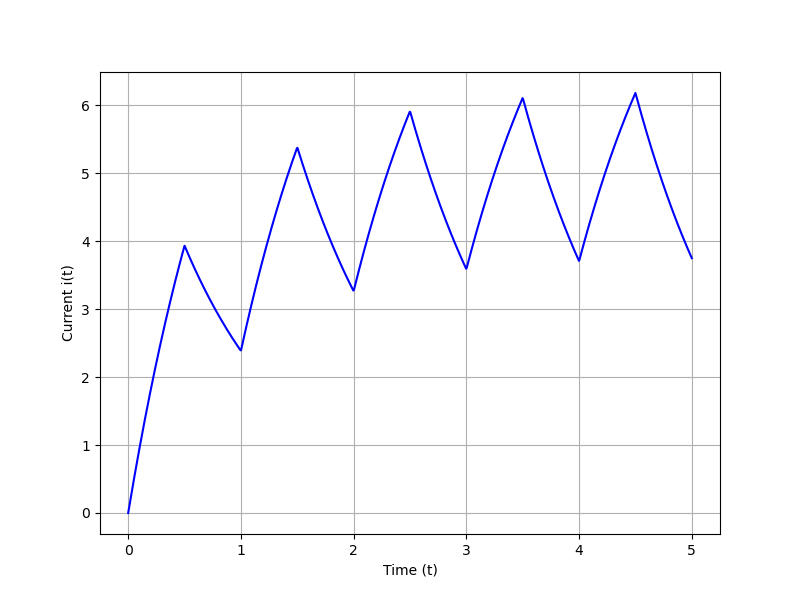
\includegraphics[width=\columnwidth]{sections/3_plot.png}
  \caption{Current Response for $R=1\Omega$, $L=1H$, and $\alpha=0.5$}
  \end{figure}
\end{multicols}

\newpage
{\color{gray}\hrule}
\begin{center}
\section{The Numerical Solution}
\bigskip
\end{center}
{\color{gray}\hrule}
\begin{multicols}{2}

\subsection{Trapezoidal Rule}
For a differential equation $$\frac{dy}{dx} = f(x,y)$$ whose solution is $y(x)$, the update equation for trapezoidal method is given by:
\begin{align}
    y_{n+1} = y_n + \frac{h}{2}\left[ f(x_n,y_n) + f(x_{n+1},_{n+1}) \right]
\end{align}
\subsection{Derivation of Update Equation}
To solve the differential equation numerically using the trapezoidal method, we discretize it as:
\begin{equation}
L \frac{I_{n+1} - I_n}{\Delta t} + R \frac{I_{n+1} + I_n}{2} = \frac{V_{n+1} + V_n}{2}
\end{equation}
Rearranging to isolate $I_{n+1}$:
\begin{equation}
L \frac{I_{n+1} - I_n}{\Delta t} = \frac{V_{n+1} + V_n}{2} - R \frac{I_{n+1} + I_n}{2}
\end{equation}
\begin{equation}
I_{n+1} \left( \frac{L}{\Delta t} + \frac{R}{2} \right) = I_n \left( \frac{L}{\Delta t} - \frac{R}{2} \right) + \frac{V_{n+1} + V_n}{2}
\end{equation}
Defining:
\begin{align}
A &= \frac{2L - R \Delta t}{2L + R \Delta t} \\
B &= \frac{\Delta t}{2L + R \Delta t}
\end{align}
The iterative formula becomes:
\begin{equation}
I_{n+1} = A I_n + B (V_{n+1} + V_n)
\end{equation}
\subsection{Why Trapezoidal?}
\begin{enumerate}
    \item Trapezoidal Rule is a popular method that is most used to solve real-world problems.
    \item It is an A-stable numerical method.
    \item Forward Euler and Backward Euler methods are first-order accurate, whereas Trapezoidal Rule is second-order accurate.
\end{enumerate}

\subsection{The Code}
\begin{lstlisting}[caption={Code for Numerical Analysis}]
import numpy as np
import matplotlib.pyplot as plt

def square_wave(t, T, alpha):
    return np.array([10 if (time % T) < (alpha * T) else 0 for time in t])

def rl_circuit_response(R, L, T, alpha, t_end, dt=0.00005):
    t = np.arange(0, t_end, dt)
    V = square_wave(t, T, alpha)
    I = np.zeros(len(t))
    A = (2 * L - R * dt) / (2 * L + R * dt)
    B = dt / (2 * L + R * dt)
    for i in range(1, len(t)):
        I[i] = A * I[i - 1] + B * (V[i] + V[i - 1])
    plt.figure(figsize=(10, 5))
    plt.plot(t, I, label="Current (I)")
    plt.xlabel("Time (s)")
    plt.ylabel("Current (A)")
    plt.grid(True)
    plt.legend()
    plt.show()

R = 1
L = 1
T = 1
alpha = 0.5
t_end = 5
dt = 0.00005

rl_circuit_response(R, L, T, alpha, t_end, dt)

\end{lstlisting}

The output generated by the above code is:
\begin{figure}[H]
  \centering
  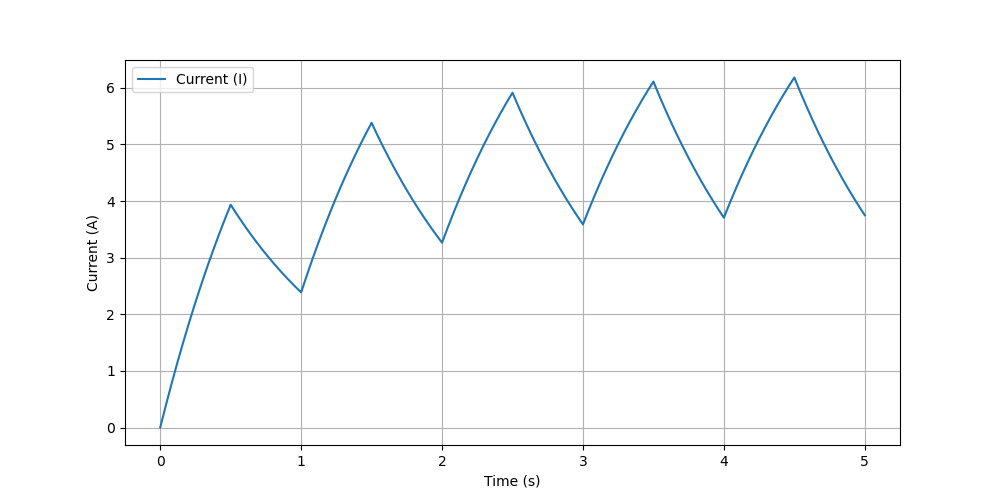
\includegraphics[width=\columnwidth]{sections/4_og.png}
  \caption{Current Response for $R=1\Omega$, $L=1H$, $T=1s$, and $\alpha=0.5$}
\end{figure}

\end{multicols}

\newpage
{\color{gray}\hrule}
\begin{center}
\section{Comparison of Solutions}
\bigskip
\end{center}
{\color{gray}\hrule}
\begin{multicols}{2}

\begin{enumerate}
    \item The response of the series RL circuit to a square wave input was computed using both numerical and analytical methods. 
    \item The numerical solution was obtained by solving the differential equation using the Trapezoidal Rule, while the analytical solution was derived using the Fourier series representation of the input signal.
    \item Upon plotting the results from both methods, it was observed that the numerical and analytical solutions produced identical waveforms. 
\end{enumerate}
\begin{figure}[H]
  \centering
  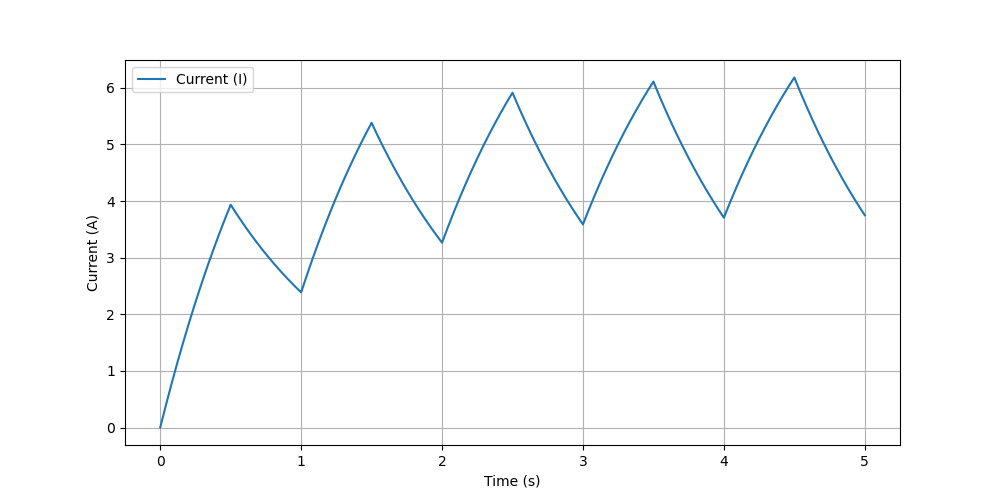
\includegraphics[width=\columnwidth]{sections/4_og.png}
  \caption{Response Obtained via Numerical Method}
\end{figure}
\begin{figure}[H]
  \centering
  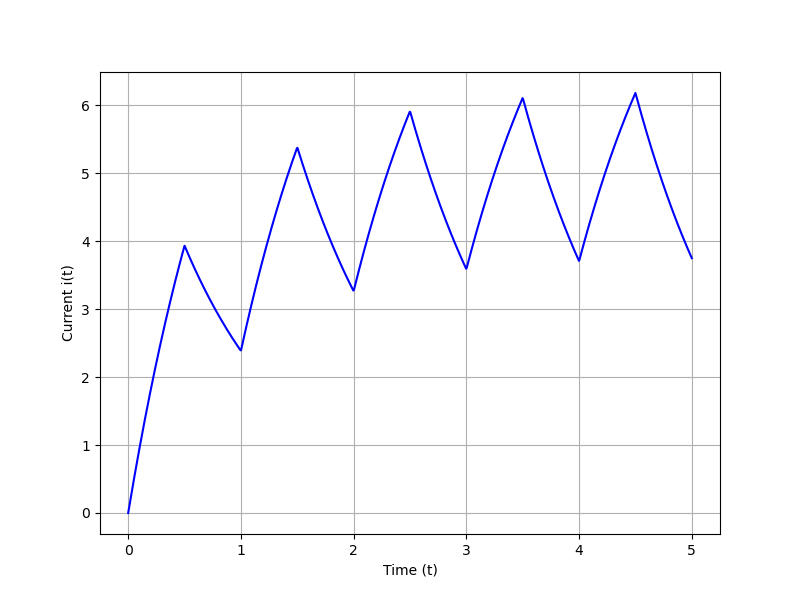
\includegraphics[width=\columnwidth]{sections/5_Analytical.png}
  \caption{Response Obtained via Analytical Method}
\end{figure}
This indicates that the numerical integration method accurately approximates the theoretical response of the circuit.

\end{multicols}

\newpage
{\color{gray}\hrule}
\begin{center}
\section{Analysis of the Response}
\bigskip
\end{center}
{\color{gray}\hrule}
\begin{multicols}{2}

Following is an analysis that details how the current response of the series $RL$ circuit to the given input wave varies as $R$, $L$, and $\alpha$ change.

\subsection{Case I: $T=\tau$}
\begin{enumerate}
    \item We can note moderate transient effects.
    \item The current tries to reach to its steady-state value each time the voltage is high ($10V$).
    \item When the voltage is low ($0V$), these attempts cease and resume only when the high voltage is achieved again.
    \item As $\alpha$ increases, we can note that the variations in current decrease, owing to the fact that the 'ON' period of the input signal is longer, and thus aids in approaching the steady-state.
\end{enumerate}
All these can be realised in the plot given below: \\
\begin{figure}[H]
  \centering
  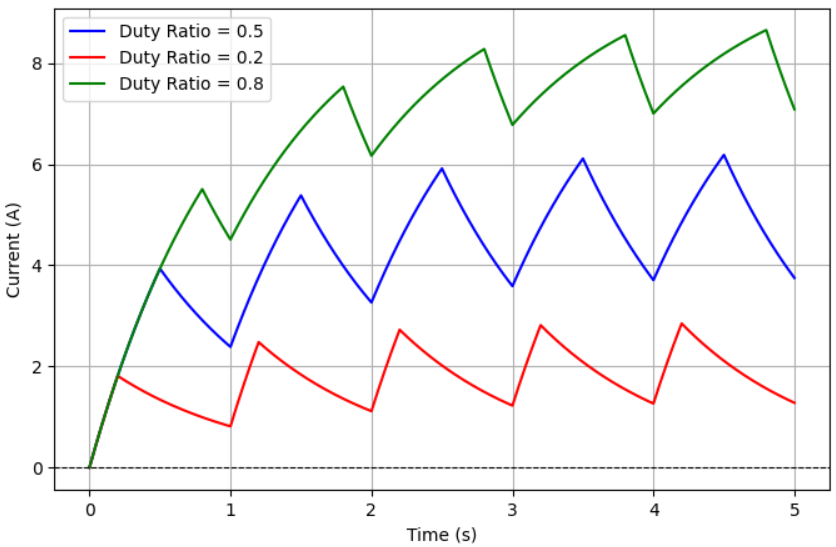
\includegraphics[width=\columnwidth]{sections/6_case1.png}
  \caption{Numerical Current Response for $R=1\Omega$, $L=1H$, and $T=1s$}
\end{figure}
\begin{figure}[H]
  \centering
  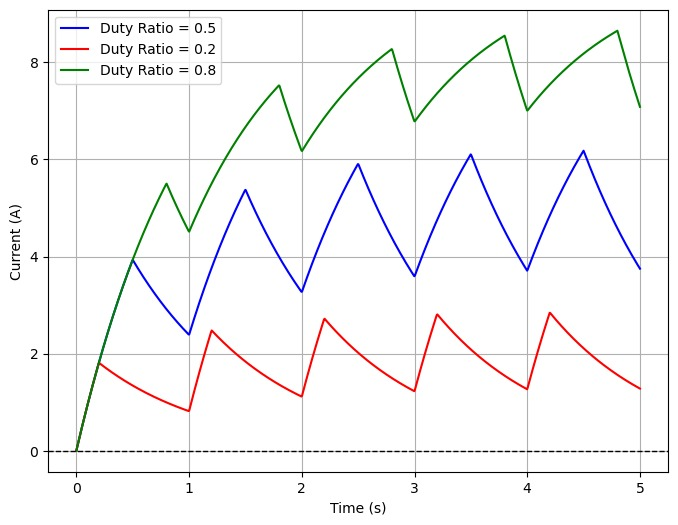
\includegraphics[width=\columnwidth]{sections/case1a.png}
  \caption{Analytical Current Response for $R=1\Omega$, $L=1H$, and $T=1s$}
\end{figure}

\subsection{Case II: $T>\tau$}
\begin{enumerate}
    \item We can note fast transient effects.
    \item The resistor dominates the circuit, and affects its behaviour accordingly.
    \item The current response closely resembles the input voltage wave (regardless of $\alpha$). This is due to the low time constant, which enables the $RL$ circuit to attain steady state current fast.
\end{enumerate}
All these can be realised in the plot given below: \\
\begin{figure}[H]
  \centering
  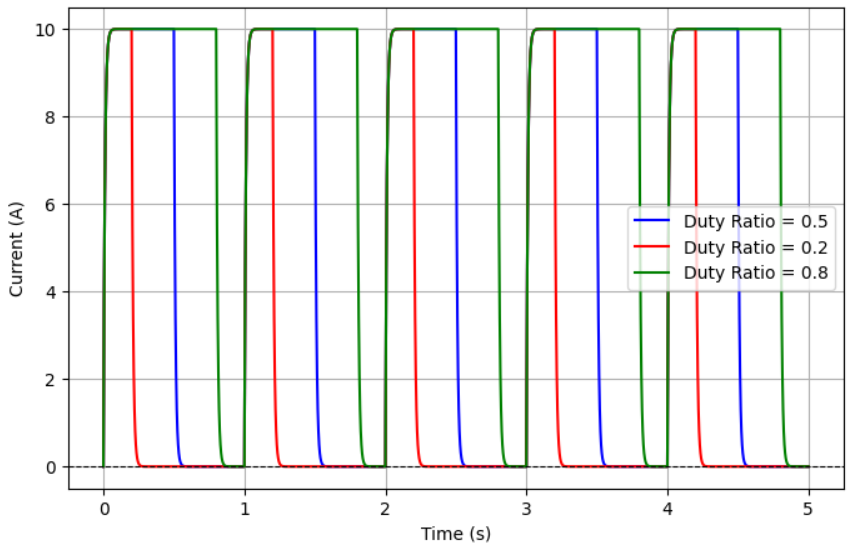
\includegraphics[width=\columnwidth]{sections/6_case2.png}
  \caption{Numerical Current Response for $R=1\Omega$, $L=0.01H$, and $T=1s$}
\end{figure}
\begin{figure}[H]
  \centering
  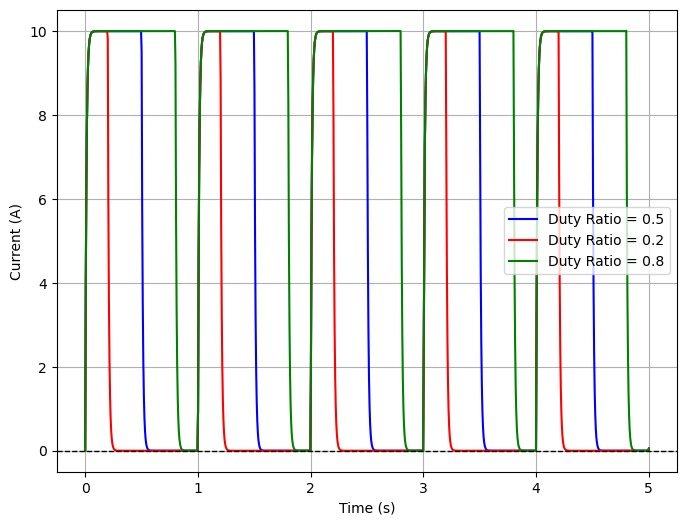
\includegraphics[width=\columnwidth]{sections/case3a.png}
  \caption{Analytical Current Response for $R=1\Omega$, $L=0.01H$, and $T=1s$}
\end{figure}

\subsection{Case III: $T<\tau$}
\begin{enumerate}
    \item We can note a slow transient response.
    \item The inductor dominates the circuit, and affects its behaviour accordingly.
    \item The current struggles to rise at each high voltage ($10V$) due to the inductive nature of the circuit.
    \item As $\alpha$ increases, the current ramps up faster each time the input voltage is high. The current vs. time graph tends to a straight line.
\end{enumerate}
All these can be realised in the plot given below: \\
\begin{figure}[H]
  \centering
  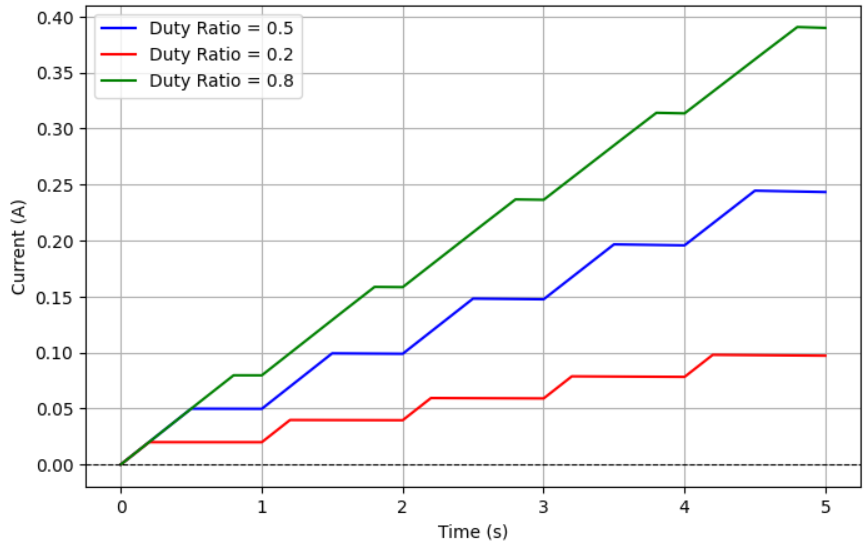
\includegraphics[width=\columnwidth]{sections/6_case3.png}
  \caption{Numerical Current Response for $R=1\Omega$, $L=100H$, and $T=1s$}
\end{figure}
\begin{figure}[H]
  \centering
  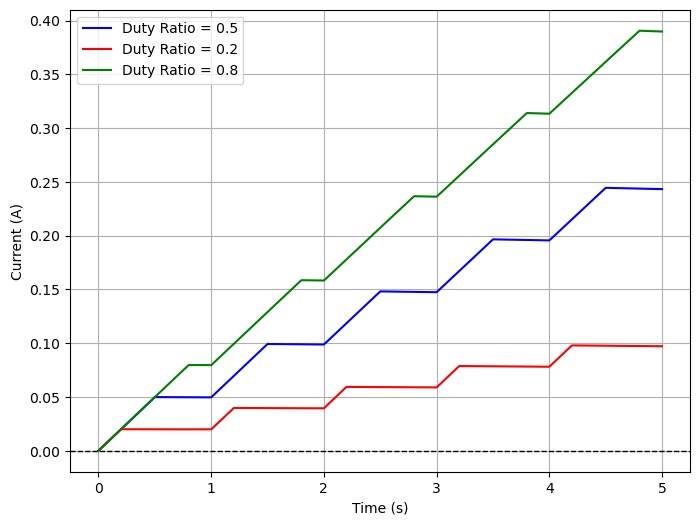
\includegraphics[width=\columnwidth]{sections/case2a.png}
  \caption{Analytical Current Response for $R=1\Omega$, $L=100H$, and $T=1s$}
\end{figure}

\end{multicols}



\newpage
{\color{gray}\hrule}
\begin{center}
\section{Fourier Analysis of Current}
\bigskip
\end{center}
{\color{gray}\hrule}
\begin{multicols}{2}
\subsection{Fourier Transform and Frequency Spectrum}
After calculating the current $I(t)$, we apply the Discrete Fourier Transform (DFT) using the Fast Fourier Transform (FFT) algorithm:
\begin{equation}
I_{\text{FFT}}(k) = \sum_{n=0}^{N-1} I_n e^{-j \frac{2 \pi k n}{N}}
\end{equation}
The magnitude spectrum is computed to analyze the frequency components. The frequency axis is determined as:
\begin{equation}
f_k = \frac{k}{N \Delta t}
\end{equation}
\subsection{Dominant Frequency}
The dominant frequency is the frequency with the highest magnitude in the Fourier spectrum, excluding the DC component at 0 Hz. Ideally, for a square wave with period $T$, the dominant frequency should be:
\begin{equation}
f_{\text{dominant}} \approx \frac{1}{T}
\end{equation}

\subsection{Impact of RL Circuit as Low-Pass Filter}
An RL circuit behaves as a \textbf{low-pass filter}, allowing low-frequency signals to pass while attenuating higher-frequency components. The cutoff frequency is given by:
\begin{equation}
f_c = \frac{R}{2 \pi L}
\end{equation}
For the given parameters:
\begin{equation}
R = 1 \, \Omega, \quad L = 1 \, \text{H} \implies f_c \approx 0.01 \, \text{Hz}
\end{equation}
When the cutoff frequency is much lower than the fundamental frequency of the square wave ($f_{\text{fundamental}} = \frac{1}{T}$), the higher harmonics of the square wave are heavily attenuated. 

\subsection{Why Dominant Frequency is Lower for High-Frequency Input}
When the input square wave has a high frequency, most of its harmonic components lie above the cutoff frequency and are significantly attenuated. As a result, the observed dominant frequency in the current response is much lower than the fundamental frequency of the input square wave:
\begin{equation}
f_{\text{dominant}} \ll \frac{1}{T} \quad \text{when } f_{\text{fundamental}} \gg f_c
\end{equation}

\subsection{Example: High-Frequency Square Wave Attenuation}
Consider an example where:
\begin{itemize}
    \item Period of the square wave: $T = 0.01 \, \text{s} \implies f_{\text{fundamental}} = 100 \, \text{Hz}$
    \item Cutoff frequency of the RL circuit: $f_c \approx 0.01 \, \text{Hz}$
\end{itemize}
Since the square wave's fundamental frequency is much higher than the cutoff frequency, the RL circuit strongly attenuates the harmonics. As a result, the dominant frequency observed in the current is not 100 Hz but a much lower value, approximately equal to the cutoff frequency:
\begin{equation}
f_{\text{dominant}} \approx 0.01 \, \text{Hz}
\end{equation}
This confirms that the RL circuit acts as a low-pass filter, suppressing higher frequencies and causing the dominant frequency to be much lower than expected.
\begin{figure}[H]
  \centering
  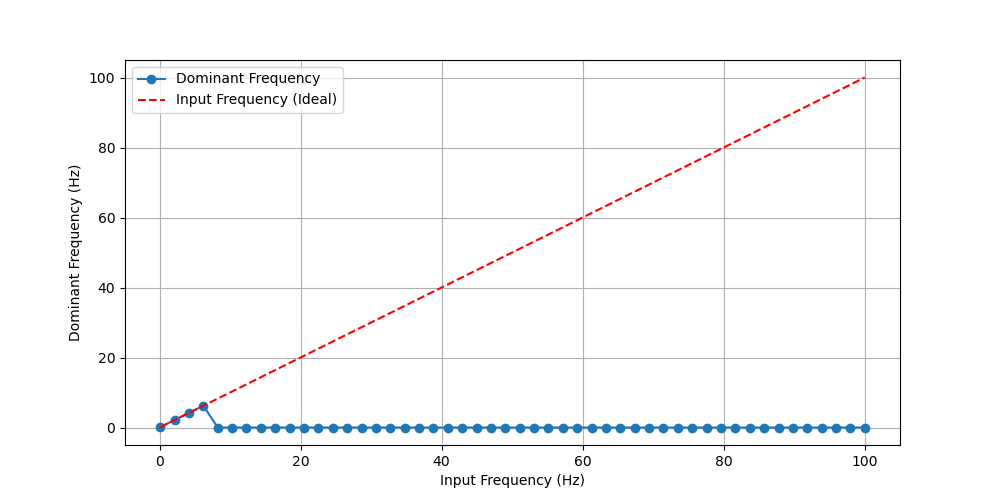
\includegraphics[width=\columnwidth]{sections/dominantfreq.png}
  \caption{Frequency vs Dominant Frequency of $R=1\Omega$, $L=1H$}
\end{figure}
\begin{figure}[H]
  \centering
  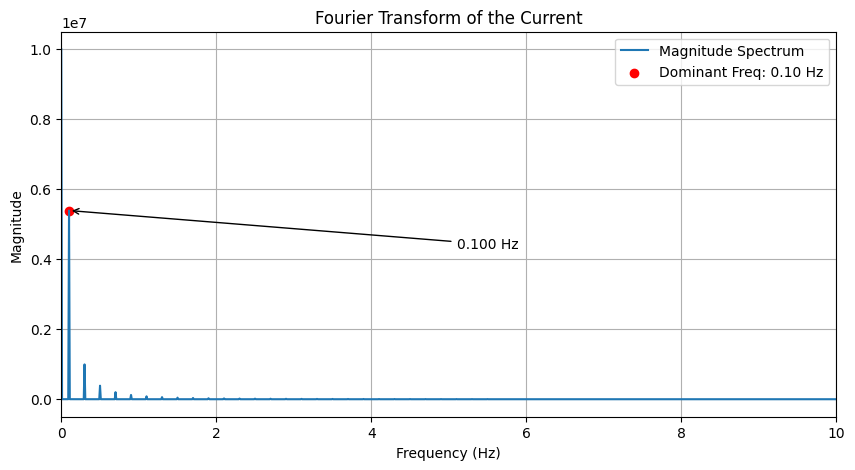
\includegraphics[width=\columnwidth]{sections/fourier_transform.png}
  \caption{Plot of Fourier coefficients of current function when $R=1\Omega$, $L=1H$, and $T=10s$}
\end{figure}
\end{multicols}

\newpage
{\color{gray}\hrule}
\begin{center}
\section{Summary and Conclusion}
\bigskip
\end{center}
{\color{gray}\hrule}
\vspace{0.5cm}
\begin{enumerate}
    \item The given input wave has been successfully decomposed into its Fourier Series expression.
\begin{equation*}
v(t) = 10\alpha + \sum_{n=1}^{\infty} \Bigg[ \frac{10 \sin (2 \pi n \alpha)}{\pi n} \cos\left(\frac{2\pi n}{T} t \right) + \frac{10}{\pi n} (1 - \cos (2 \pi n \alpha)) \sin\left(\frac{2\pi n}{T} t \right) \Bigg]
\end{equation*}
    \item The differential equation was deduced, and it was used to solve for the current response of the $RL$ circuit analytically and via a numerical method (trapezoidal rule).
\begin{align*}
i(t) &= \frac{a_0}{R} \left(1-e^{\frac{-R}{L}t} \right) + \sum_{n=1}^{\infty} \Bigg( \frac{\sqrt{a_n^2+b_n^2}}{\sqrt{R^2+(n\omega_0L)^2}} \cos(n\omega_0t-\phi-\theta) - e^{\frac{-R}{L}t} \frac{\cos(\phi+\theta)}{\sqrt{R^2+(n\omega_0L)^2}} \Bigg)
\end{align*}
where
\begin{align*}
a_0&=10\alpha\\
\phi &= \arctan{\frac{b_n}{a_n}}\\
\theta&=tan^{-1}\left(\frac{n\omega_0L}{R}\right)\\
a_n&=\frac{10 \sin 2 \pi n \alpha}{\pi n} \\
b_n&=\left( \frac{10}{ \pi n} \right) (1 - \cos 2 \pi n \alpha)
\end{align*}
    \item Responses obtained through both methods were compared, and furthur analysis was done to understand the nature of the response and how it varies with $R$, $L$, and $\alpha$.
    \item Finally, a Fourier analysis was done on the current response, and other related characteristics were explored.
    \item Codes for all generated plots can be found at this \href{https://github.com/mandara-h/EE1060}{GitHub repository}.
\end{enumerate}


\newpage
\begin{thebibliography}{9}
    \bibitem{latex1} Lectures of Differential Equations and Transform Techniques, EE1060 (Jan-May 2025)
    \bibitem{latex2} Lectures of Circuits and Network Analysis, EE1101 (Jul-Nov 2024)
    \bibitem{latex3} \href{https://homepage.math.uiowa.edu/~atkinson/papers/NAODE_Book.pdf}{Numerical Solution of Ordinary Differential Equations} by K. Atkinson, W. Han, and D. Stewart
    \bibitem{latex4} \href{https://en.wikipedia.org/wiki/Trapezoidal_rule_(differential_equations)}{Wikipedia page} on using Trapezoidal Method to Solve Differential Equations
    \bibitem{latex5} \href{https://books.google.co.in/books?id=7Zofw3SFTWIC&q=%22Trapezoidal+rule%22&redir_esc=y#v=snippet&q=%22Trapezoidal%20rule%22&f=false}{A First Course in the Numerical Analysis of Differential Equations} by Arieh Iserles
    \bibitem{latex6} \href{https://www.cs.usask.ca/~spiteri/M314/notes/AP/chap3.pdf}{Lecture Notes} for the course M314 offered at University of Saskatchewan
\end{thebibliography}
\end{document}
